% AUTO-GENERATED by run_dose_response_benchmark.py -- DO NOT EDIT.
% Regenerate with:  python run_dose_response_benchmark.py --stage tables
%

\subsection{\emph{bowl-shaped} plate effects (bowl (negatives unaffected))}


\subsubsection{$d_{\max}$ errors}

\begin{figure*}[!htbp]
  \centering
  \begin{subfigure}[c]{0.05\textwidth}
    ~
  \end{subfigure}
  %
  \begin{subfigure}[c]{0.40\textwidth}
    \centering
    ~~\textbf{Mild plate effects}
  \end{subfigure}
  %
  \begin{subfigure}[c]{0.40\textwidth}
    \centering
    ~~\textbf{Strong plate effects}
  \end{subfigure}

  \begin{subfigure}[c]{0.05\textwidth}
    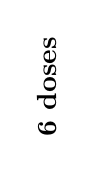
\begin{tikzpicture}
      \node[rotate=90] {\textbf{6 doses}};
    \end{tikzpicture}
  \end{subfigure}
  %
  \begin{subfigure}[c]{0.40\textwidth}
    \includegraphics[width=\textwidth]{figures/dose-response-d_diff-1-2-3-6doses-dil18-bowl-0.055.png}
  \end{subfigure}
  %
  \begin{subfigure}[c]{0.40\textwidth}
    \centering
    \includegraphics[width=\textwidth]{figures/dose-response-d_diff-1-2-3-6doses-dil18-bowl-0.085.png}
  \end{subfigure}

  \begin{subfigure}[c]{0.05\textwidth}
    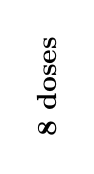
\begin{tikzpicture}
      \node[rotate=90] {\textbf{8 doses}};
    \end{tikzpicture}
  \end{subfigure}
  %
  \begin{subfigure}[c]{0.40\textwidth}
    \includegraphics[width=\textwidth]{figures/dose-response-d_diff-1-2-3-8doses-dil8-bowl-0.055.png}
  \end{subfigure}
  %
  \begin{subfigure}[c]{0.40\textwidth}
    \centering
    \includegraphics[width=\textwidth]{figures/dose-response-d_diff-1-2-3-8doses-dil8-bowl-0.085.png}
  \end{subfigure}

  \begin{subfigure}[c]{0.05\textwidth}
    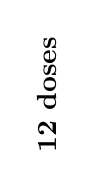
\begin{tikzpicture}
      \node[rotate=90] {\textbf{12 doses}};
    \end{tikzpicture}
  \end{subfigure}
  %
  \begin{subfigure}[c]{0.40\textwidth}
    \includegraphics[width=\textwidth]{figures/dose-response-d_diff-1-2-3-12doses-dil4-bowl-0.055.png}
  \end{subfigure}
  %
  \begin{subfigure}[c]{0.40\textwidth}
    \centering
    \includegraphics[width=\textwidth]{figures/dose-response-d_diff-1-2-3-12doses-dil4-bowl-0.085.png}
  \end{subfigure}

  \caption{Mean absolute difference between expected and obtained heights ($d_{\max}$) for dose-response curves using various numbers of doses, replicates, and \emph{bowl-shaped} plate-effect strengths. The 4PL sigmoid curves were fitted using compound data and 4 negative controls such that their mean was equal to the mean of the 20 negative controls on the plate. *** indicates $p\leq10^{-43}$.}
\end{figure*}

\begin{table}[H]
  \caption{%
    $d_{max}$ error overview for \emph{bowl-shaped} plate-effect strengths. Values are mean absolute differences in fitted $d_{max}$ across compounds. Best (lowest) value per row is \textbf{bolded}.
  }
  \label{tab:dr-overview-dmax-bowl}
  \centering
  \input{tables/dr-overview-dmax-bowl}
\end{table}


\clearpage
\subsubsection{Relative IC$_{50}$/EC$_{50}$ errors}

\begin{figure*}[!htbp]
  \centering
  \begin{subfigure}[c]{0.05\textwidth}
    ~
  \end{subfigure}
  %
  \begin{subfigure}[c]{0.40\textwidth}
    \centering
    ~~\textbf{Mild plate effects}
  \end{subfigure}
  %
  \begin{subfigure}[c]{0.40\textwidth}
    \centering
    ~~\textbf{Strong plate effects}
  \end{subfigure}

  \begin{subfigure}[c]{0.05\textwidth}
    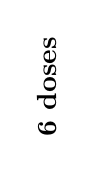
\begin{tikzpicture}
      \node[rotate=90] {\textbf{6 doses}};
    \end{tikzpicture}
  \end{subfigure}
  %
  \begin{subfigure}[c]{0.40\textwidth}
    \includegraphics[width=\textwidth]{figures/dose-response-relic50-1-2-3-6doses-dil18-bowl-0.055.png}
  \end{subfigure}
  %
  \begin{subfigure}[c]{0.40\textwidth}
    \centering
    \includegraphics[width=\textwidth]{figures/dose-response-relic50-1-2-3-6doses-dil18-bowl-0.085.png}
  \end{subfigure}

  \begin{subfigure}[c]{0.05\textwidth}
    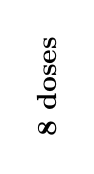
\begin{tikzpicture}
      \node[rotate=90] {\textbf{8 doses}};
    \end{tikzpicture}
  \end{subfigure}
  %
  \begin{subfigure}[c]{0.40\textwidth}
    \includegraphics[width=\textwidth]{figures/dose-response-relic50-1-2-3-8doses-dil8-bowl-0.055.png}
  \end{subfigure}
  %
  \begin{subfigure}[c]{0.40\textwidth}
    \centering
    \includegraphics[width=\textwidth]{figures/dose-response-relic50-1-2-3-8doses-dil8-bowl-0.085.png}
  \end{subfigure}

  \begin{subfigure}[c]{0.05\textwidth}
    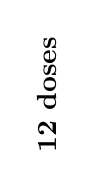
\begin{tikzpicture}
      \node[rotate=90] {\textbf{12 doses}};
    \end{tikzpicture}
  \end{subfigure}
  %
  \begin{subfigure}[c]{0.40\textwidth}
    \includegraphics[width=\textwidth]{figures/dose-response-relic50-1-2-3-12doses-dil4-bowl-0.055.png}
  \end{subfigure}
  %
  \begin{subfigure}[c]{0.40\textwidth}
    \centering
    \includegraphics[width=\textwidth]{figures/dose-response-relic50-1-2-3-12doses-dil4-bowl-0.085.png}
  \end{subfigure}

  \caption{Relative IC$_{50}$/EC$_{50}$ error for dose-response curves using various numbers of doses, replicates, and \emph{bowl-shaped} plate-effect strengths. *** indicates $p\leq10^{-43}$.}
\end{figure*}

\begin{table}[H]
  \caption{%
    Relative IC$_{50}$/EC$_{50}$ MSE overview for \emph{bowl-shaped} plate-effect strengths. Best (lowest) value per row is \textbf{bolded}.
  }
  \label{tab:dr-overview-rel-ic50-bowl}
  \centering
  \input{tables/dr-overview-rel-ic50-bowl}
\end{table}


\clearpage
\subsubsection{Absolute IC$_{50}$/EC$_{50}$ errors}

\begin{figure*}[!htbp]
  \centering
  \begin{subfigure}[c]{0.05\textwidth}
    ~
  \end{subfigure}
  %
  \begin{subfigure}[c]{0.40\textwidth}
    \centering
    ~~\textbf{Mild plate effects}
  \end{subfigure}
  %
  \begin{subfigure}[c]{0.40\textwidth}
    \centering
    ~~\textbf{Strong plate effects}
  \end{subfigure}

  \begin{subfigure}[c]{0.05\textwidth}
    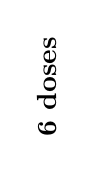
\begin{tikzpicture}
      \node[rotate=90] {\textbf{6 doses}};
    \end{tikzpicture}
  \end{subfigure}
  %
  \begin{subfigure}[c]{0.40\textwidth}
    \includegraphics[width=\textwidth]{figures/dose-response-absic50-1-2-3-6doses-dil18-bowl-0.055.png}
  \end{subfigure}
  %
  \begin{subfigure}[c]{0.40\textwidth}
    \centering
    \includegraphics[width=\textwidth]{figures/dose-response-absic50-1-2-3-6doses-dil18-bowl-0.085.png}
  \end{subfigure}

  \begin{subfigure}[c]{0.05\textwidth}
    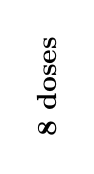
\begin{tikzpicture}
      \node[rotate=90] {\textbf{8 doses}};
    \end{tikzpicture}
  \end{subfigure}
  %
  \begin{subfigure}[c]{0.40\textwidth}
    \includegraphics[width=\textwidth]{figures/dose-response-absic50-1-2-3-8doses-dil8-bowl-0.055.png}
  \end{subfigure}
  %
  \begin{subfigure}[c]{0.40\textwidth}
    \centering
    \includegraphics[width=\textwidth]{figures/dose-response-absic50-1-2-3-8doses-dil8-bowl-0.085.png}
  \end{subfigure}

  \begin{subfigure}[c]{0.05\textwidth}
    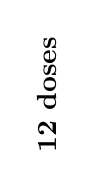
\begin{tikzpicture}
      \node[rotate=90] {\textbf{12 doses}};
    \end{tikzpicture}
  \end{subfigure}
  %
  \begin{subfigure}[c]{0.40\textwidth}
    \includegraphics[width=\textwidth]{figures/dose-response-absic50-1-2-3-12doses-dil4-bowl-0.055.png}
  \end{subfigure}
  %
  \begin{subfigure}[c]{0.40\textwidth}
    \centering
    \includegraphics[width=\textwidth]{figures/dose-response-absic50-1-2-3-12doses-dil4-bowl-0.085.png}
  \end{subfigure}

  \caption{Absolute IC$_{50}$/EC$_{50}$ error for dose-response curves using various numbers of doses, replicates, and \emph{bowl-shaped} plate-effect strengths. *** indicates $p\leq10^{-43}$.}
\end{figure*}

\begin{table}[H]
  \caption{%
    Absolute IC$_{50}$/EC$_{50}$ error overview for \emph{bowl-shaped} plate-effect strengths. Values are mean squared absolute IC$_{50}$/EC$_{50}$ estimation errors across compounds. Best (lowest) value per row is \textbf{bolded}.
  }
  \label{tab:dr-overview-abs-ic50-bowl}
  \centering
  \input{tables/dr-overview-abs-ic50-bowl}
\end{table}


\clearpage
\subsubsection{Residuals}

\begin{figure*}[!htbp]
  \centering
  \begin{subfigure}[c]{0.05\textwidth}
    ~
  \end{subfigure}
  %
  \begin{subfigure}[c]{0.40\textwidth}
    \centering
    ~~\textbf{Mild plate effects}
  \end{subfigure}
  %
  \begin{subfigure}[c]{0.40\textwidth}
    \centering
    ~~\textbf{Strong plate effects}
  \end{subfigure}

  \begin{subfigure}[c]{0.05\textwidth}
    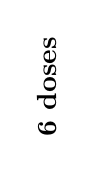
\begin{tikzpicture}
      \node[rotate=90] {\textbf{6 doses}};
    \end{tikzpicture}
  \end{subfigure}
  %
  \begin{subfigure}[c]{0.40\textwidth}
    \includegraphics[width=\textwidth]{figures/residuals-1-2-3-6doses-dil18-bowl-0.055.png}
  \end{subfigure}
  %
  \begin{subfigure}[c]{0.40\textwidth}
    \centering
    \includegraphics[width=\textwidth]{figures/residuals-1-2-3-6doses-dil18-bowl-0.085.png}
  \end{subfigure}

  \begin{subfigure}[c]{0.05\textwidth}
    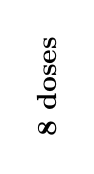
\begin{tikzpicture}
      \node[rotate=90] {\textbf{8 doses}};
    \end{tikzpicture}
  \end{subfigure}
  %
  \begin{subfigure}[c]{0.40\textwidth}
    \includegraphics[width=\textwidth]{figures/residuals-1-2-3-8doses-dil8-bowl-0.055.png}
  \end{subfigure}
  %
  \begin{subfigure}[c]{0.40\textwidth}
    \centering
    \includegraphics[width=\textwidth]{figures/residuals-1-2-3-8doses-dil8-bowl-0.085.png}
  \end{subfigure}

  \begin{subfigure}[c]{0.05\textwidth}
    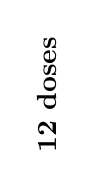
\begin{tikzpicture}
      \node[rotate=90] {\textbf{12 doses}};
    \end{tikzpicture}
  \end{subfigure}
  %
  \begin{subfigure}[c]{0.40\textwidth}
    \includegraphics[width=\textwidth]{figures/residuals-1-2-3-12doses-dil4-bowl-0.055.png}
  \end{subfigure}
  %
  \begin{subfigure}[c]{0.40\textwidth}
    \centering
    \includegraphics[width=\textwidth]{figures/residuals-1-2-3-12doses-dil4-bowl-0.085.png}
  \end{subfigure}

  \caption{Residuals (MSE between expected and obtained responses) for dose-response simulations using various numbers of doses, replicates, and \emph{bowl-shaped} plate-effect strengths. *** indicates $p\leq10^{-43}$.}
\end{figure*}

\begin{table}[H]
  \caption{%
    Residual MSE overview for \emph{bowl-shaped} plate-effect strengths. Best (lowest) value per row is \textbf{bolded}.
  }
  \label{tab:dr-overview-residuals-bowl}
  \centering
  \input{tables/dr-overview-residuals-bowl}
\end{table}


\clearpage
\subsubsection{Fraction of poor fits (low $R^2$)}

\begin{figure*}[!htbp]
  \centering
  \begin{subfigure}[c]{0.05\textwidth}
    ~
  \end{subfigure}
  %
  \begin{subfigure}[c]{0.40\textwidth}
    \centering
    ~~\textbf{Mild plate effects}
  \end{subfigure}
  %
  \begin{subfigure}[c]{0.40\textwidth}
    \centering
    ~~\textbf{Strong plate effects}
  \end{subfigure}

  \begin{subfigure}[c]{0.05\textwidth}
    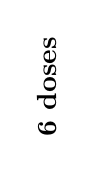
\begin{tikzpicture}
      \node[rotate=90] {\textbf{6 doses}};
    \end{tikzpicture}
  \end{subfigure}
  %
  \begin{subfigure}[c]{0.40\textwidth}
    \includegraphics[width=\textwidth]{figures/percentage-low-r2-curves-1-2-3-6doses-dil18-bowl-0.055.png}
  \end{subfigure}
  %
  \begin{subfigure}[c]{0.40\textwidth}
    \centering
    \includegraphics[width=\textwidth]{figures/percentage-low-r2-curves-1-2-3-6doses-dil18-bowl-0.085.png}
  \end{subfigure}

  \begin{subfigure}[c]{0.05\textwidth}
    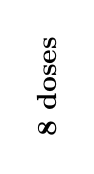
\begin{tikzpicture}
      \node[rotate=90] {\textbf{8 doses}};
    \end{tikzpicture}
  \end{subfigure}
  %
  \begin{subfigure}[c]{0.40\textwidth}
    \includegraphics[width=\textwidth]{figures/percentage-low-r2-curves-1-2-3-8doses-dil8-bowl-0.055.png}
  \end{subfigure}
  %
  \begin{subfigure}[c]{0.40\textwidth}
    \centering
    \includegraphics[width=\textwidth]{figures/percentage-low-r2-curves-1-2-3-8doses-dil8-bowl-0.085.png}
  \end{subfigure}

  \begin{subfigure}[c]{0.05\textwidth}
    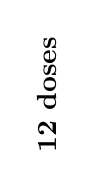
\begin{tikzpicture}
      \node[rotate=90] {\textbf{12 doses}};
    \end{tikzpicture}
  \end{subfigure}
  %
  \begin{subfigure}[c]{0.40\textwidth}
    \includegraphics[width=\textwidth]{figures/percentage-low-r2-curves-1-2-3-12doses-dil4-bowl-0.055.png}
  \end{subfigure}
  %
  \begin{subfigure}[c]{0.40\textwidth}
    \centering
    \includegraphics[width=\textwidth]{figures/percentage-low-r2-curves-1-2-3-12doses-dil4-bowl-0.085.png}
  \end{subfigure}

  \caption{Percentage of dose-response curves with low-quality ($R^2 < 80\%$) using various numbers of doses, replicates, and \emph{bowl-shaped} plate-effect strengths. The 4PL sigmoid curves were fitted using compound data and 4 negative controls such that their mean was equal to the mean of the 20 negative controls on the plate.}
\end{figure*}

\clearpage
\subsection{\emph{bowl-shaped} plate effects (bowl (negatives affected))}


\subsubsection{$d_{\max}$ errors}

\begin{figure*}[!htbp]
  \centering
  \begin{subfigure}[c]{0.05\textwidth}
    ~
  \end{subfigure}
  %
  \begin{subfigure}[c]{0.40\textwidth}
    \centering
    ~~\textbf{Mild plate effects}
  \end{subfigure}
  %
  \begin{subfigure}[c]{0.40\textwidth}
    \centering
    ~~\textbf{Strong plate effects}
  \end{subfigure}

  \begin{subfigure}[c]{0.05\textwidth}
    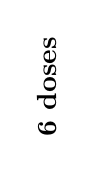
\begin{tikzpicture}
      \node[rotate=90] {\textbf{6 doses}};
    \end{tikzpicture}
  \end{subfigure}
  %
  \begin{subfigure}[c]{0.40\textwidth}
    \includegraphics[width=\textwidth]{figures/dose-response-d_diff-1-2-3-6doses-dil18-bowl-neg-controls-0.055.png}
  \end{subfigure}
  %
  \begin{subfigure}[c]{0.40\textwidth}
    \centering
    \includegraphics[width=\textwidth]{figures/dose-response-d_diff-1-2-3-6doses-dil18-bowl-neg-controls-0.085.png}
  \end{subfigure}

  \begin{subfigure}[c]{0.05\textwidth}
    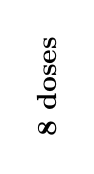
\begin{tikzpicture}
      \node[rotate=90] {\textbf{8 doses}};
    \end{tikzpicture}
  \end{subfigure}
  %
  \begin{subfigure}[c]{0.40\textwidth}
    \includegraphics[width=\textwidth]{figures/dose-response-d_diff-1-2-3-8doses-dil8-bowl-neg-controls-0.055.png}
  \end{subfigure}
  %
  \begin{subfigure}[c]{0.40\textwidth}
    \centering
    \includegraphics[width=\textwidth]{figures/dose-response-d_diff-1-2-3-8doses-dil8-bowl-neg-controls-0.085.png}
  \end{subfigure}

  \begin{subfigure}[c]{0.05\textwidth}
    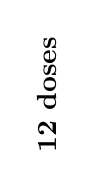
\begin{tikzpicture}
      \node[rotate=90] {\textbf{12 doses}};
    \end{tikzpicture}
  \end{subfigure}
  %
  \begin{subfigure}[c]{0.40\textwidth}
    \includegraphics[width=\textwidth]{figures/dose-response-d_diff-1-2-3-12doses-dil4-bowl-neg-controls-0.055.png}
  \end{subfigure}
  %
  \begin{subfigure}[c]{0.40\textwidth}
    \centering
    \includegraphics[width=\textwidth]{figures/dose-response-d_diff-1-2-3-12doses-dil4-bowl-neg-controls-0.085.png}
  \end{subfigure}

  \caption{Mean absolute difference between expected and obtained heights ($d_{\max}$) for dose-response curves using various numbers of doses, replicates, and \emph{bowl-shaped} plate-effect strengths. The 4PL sigmoid curves were fitted using compound data and 4 negative controls such that their mean was equal to the mean of the 20 negative controls on the plate. *** indicates $p\leq10^{-43}$.}
\end{figure*}

\begin{table}[H]
  \caption{%
    $d_{max}$ error overview for \emph{bowl-shaped} plate-effect strengths. Values are mean absolute differences in fitted $d_{max}$ across compounds. Best (lowest) value per row is \textbf{bolded}.
  }
  \label{tab:dr-overview-dmax-bowl-neg}
  \centering
  \input{tables/dr-overview-dmax-bowl-neg}
\end{table}


\clearpage
\subsubsection{Relative IC$_{50}$/EC$_{50}$ errors}

\begin{figure*}[!htbp]
  \centering
  \begin{subfigure}[c]{0.05\textwidth}
    ~
  \end{subfigure}
  %
  \begin{subfigure}[c]{0.40\textwidth}
    \centering
    ~~\textbf{Mild plate effects}
  \end{subfigure}
  %
  \begin{subfigure}[c]{0.40\textwidth}
    \centering
    ~~\textbf{Strong plate effects}
  \end{subfigure}

  \begin{subfigure}[c]{0.05\textwidth}
    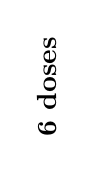
\begin{tikzpicture}
      \node[rotate=90] {\textbf{6 doses}};
    \end{tikzpicture}
  \end{subfigure}
  %
  \begin{subfigure}[c]{0.40\textwidth}
    \includegraphics[width=\textwidth]{figures/dose-response-relic50-1-2-3-6doses-dil18-bowl-neg-controls-0.055.png}
  \end{subfigure}
  %
  \begin{subfigure}[c]{0.40\textwidth}
    \centering
    \includegraphics[width=\textwidth]{figures/dose-response-relic50-1-2-3-6doses-dil18-bowl-neg-controls-0.085.png}
  \end{subfigure}

  \begin{subfigure}[c]{0.05\textwidth}
    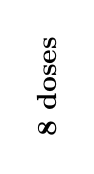
\begin{tikzpicture}
      \node[rotate=90] {\textbf{8 doses}};
    \end{tikzpicture}
  \end{subfigure}
  %
  \begin{subfigure}[c]{0.40\textwidth}
    \includegraphics[width=\textwidth]{figures/dose-response-relic50-1-2-3-8doses-dil8-bowl-neg-controls-0.055.png}
  \end{subfigure}
  %
  \begin{subfigure}[c]{0.40\textwidth}
    \centering
    \includegraphics[width=\textwidth]{figures/dose-response-relic50-1-2-3-8doses-dil8-bowl-neg-controls-0.085.png}
  \end{subfigure}

  \begin{subfigure}[c]{0.05\textwidth}
    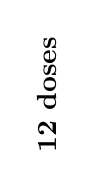
\begin{tikzpicture}
      \node[rotate=90] {\textbf{12 doses}};
    \end{tikzpicture}
  \end{subfigure}
  %
  \begin{subfigure}[c]{0.40\textwidth}
    \includegraphics[width=\textwidth]{figures/dose-response-relic50-1-2-3-12doses-dil4-bowl-neg-controls-0.055.png}
  \end{subfigure}
  %
  \begin{subfigure}[c]{0.40\textwidth}
    \centering
    \includegraphics[width=\textwidth]{figures/dose-response-relic50-1-2-3-12doses-dil4-bowl-neg-controls-0.085.png}
  \end{subfigure}

  \caption{Relative IC$_{50}$/EC$_{50}$ error for dose-response curves using various numbers of doses, replicates, and \emph{bowl-shaped} plate-effect strengths. *** indicates $p\leq10^{-43}$.}
\end{figure*}

\begin{table}[H]
  \caption{%
    Relative IC$_{50}$/EC$_{50}$ MSE overview for \emph{bowl-shaped} plate-effect strengths. Best (lowest) value per row is \textbf{bolded}.
  }
  \label{tab:dr-overview-rel-ic50-bowl-neg}
  \centering
  \input{tables/dr-overview-rel-ic50-bowl-neg}
\end{table}


\clearpage
\subsubsection{Absolute IC$_{50}$/EC$_{50}$ errors}

\begin{figure*}[!htbp]
  \centering
  \begin{subfigure}[c]{0.05\textwidth}
    ~
  \end{subfigure}
  %
  \begin{subfigure}[c]{0.40\textwidth}
    \centering
    ~~\textbf{Mild plate effects}
  \end{subfigure}
  %
  \begin{subfigure}[c]{0.40\textwidth}
    \centering
    ~~\textbf{Strong plate effects}
  \end{subfigure}

  \begin{subfigure}[c]{0.05\textwidth}
    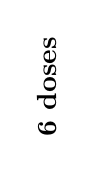
\begin{tikzpicture}
      \node[rotate=90] {\textbf{6 doses}};
    \end{tikzpicture}
  \end{subfigure}
  %
  \begin{subfigure}[c]{0.40\textwidth}
    \includegraphics[width=\textwidth]{figures/dose-response-absic50-1-2-3-6doses-dil18-bowl-neg-controls-0.055.png}
  \end{subfigure}
  %
  \begin{subfigure}[c]{0.40\textwidth}
    \centering
    \includegraphics[width=\textwidth]{figures/dose-response-absic50-1-2-3-6doses-dil18-bowl-neg-controls-0.085.png}
  \end{subfigure}

  \begin{subfigure}[c]{0.05\textwidth}
    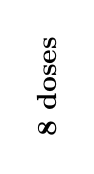
\begin{tikzpicture}
      \node[rotate=90] {\textbf{8 doses}};
    \end{tikzpicture}
  \end{subfigure}
  %
  \begin{subfigure}[c]{0.40\textwidth}
    \includegraphics[width=\textwidth]{figures/dose-response-absic50-1-2-3-8doses-dil8-bowl-neg-controls-0.055.png}
  \end{subfigure}
  %
  \begin{subfigure}[c]{0.40\textwidth}
    \centering
    \includegraphics[width=\textwidth]{figures/dose-response-absic50-1-2-3-8doses-dil8-bowl-neg-controls-0.085.png}
  \end{subfigure}

  \begin{subfigure}[c]{0.05\textwidth}
    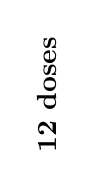
\begin{tikzpicture}
      \node[rotate=90] {\textbf{12 doses}};
    \end{tikzpicture}
  \end{subfigure}
  %
  \begin{subfigure}[c]{0.40\textwidth}
    \includegraphics[width=\textwidth]{figures/dose-response-absic50-1-2-3-12doses-dil4-bowl-neg-controls-0.055.png}
  \end{subfigure}
  %
  \begin{subfigure}[c]{0.40\textwidth}
    \centering
    \includegraphics[width=\textwidth]{figures/dose-response-absic50-1-2-3-12doses-dil4-bowl-neg-controls-0.085.png}
  \end{subfigure}

  \caption{Absolute IC$_{50}$/EC$_{50}$ error for dose-response curves using various numbers of doses, replicates, and \emph{bowl-shaped} plate-effect strengths. *** indicates $p\leq10^{-43}$.}
\end{figure*}

\begin{table}[H]
  \caption{%
    Absolute IC$_{50}$/EC$_{50}$ error overview for \emph{bowl-shaped} plate-effect strengths. Values are mean squared absolute IC$_{50}$/EC$_{50}$ estimation errors across compounds. Best (lowest) value per row is \textbf{bolded}.
  }
  \label{tab:dr-overview-abs-ic50-bowl-neg}
  \centering
  \input{tables/dr-overview-abs-ic50-bowl-neg}
\end{table}


\clearpage
\subsubsection{Residuals}

\begin{figure*}[!htbp]
  \centering
  \begin{subfigure}[c]{0.05\textwidth}
    ~
  \end{subfigure}
  %
  \begin{subfigure}[c]{0.40\textwidth}
    \centering
    ~~\textbf{Mild plate effects}
  \end{subfigure}
  %
  \begin{subfigure}[c]{0.40\textwidth}
    \centering
    ~~\textbf{Strong plate effects}
  \end{subfigure}

  \begin{subfigure}[c]{0.05\textwidth}
    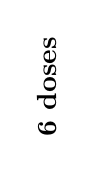
\begin{tikzpicture}
      \node[rotate=90] {\textbf{6 doses}};
    \end{tikzpicture}
  \end{subfigure}
  %
  \begin{subfigure}[c]{0.40\textwidth}
    \includegraphics[width=\textwidth]{figures/residuals-1-2-3-6doses-dil18-bowl-neg-controls-0.055.png}
  \end{subfigure}
  %
  \begin{subfigure}[c]{0.40\textwidth}
    \centering
    \includegraphics[width=\textwidth]{figures/residuals-1-2-3-6doses-dil18-bowl-neg-controls-0.085.png}
  \end{subfigure}

  \begin{subfigure}[c]{0.05\textwidth}
    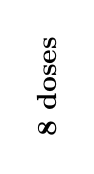
\begin{tikzpicture}
      \node[rotate=90] {\textbf{8 doses}};
    \end{tikzpicture}
  \end{subfigure}
  %
  \begin{subfigure}[c]{0.40\textwidth}
    \includegraphics[width=\textwidth]{figures/residuals-1-2-3-8doses-dil8-bowl-neg-controls-0.055.png}
  \end{subfigure}
  %
  \begin{subfigure}[c]{0.40\textwidth}
    \centering
    \includegraphics[width=\textwidth]{figures/residuals-1-2-3-8doses-dil8-bowl-neg-controls-0.085.png}
  \end{subfigure}

  \begin{subfigure}[c]{0.05\textwidth}
    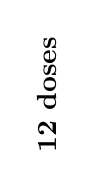
\begin{tikzpicture}
      \node[rotate=90] {\textbf{12 doses}};
    \end{tikzpicture}
  \end{subfigure}
  %
  \begin{subfigure}[c]{0.40\textwidth}
    \includegraphics[width=\textwidth]{figures/residuals-1-2-3-12doses-dil4-bowl-neg-controls-0.055.png}
  \end{subfigure}
  %
  \begin{subfigure}[c]{0.40\textwidth}
    \centering
    \includegraphics[width=\textwidth]{figures/residuals-1-2-3-12doses-dil4-bowl-neg-controls-0.085.png}
  \end{subfigure}

  \caption{Residuals (MSE between expected and obtained responses) for dose-response simulations using various numbers of doses, replicates, and \emph{bowl-shaped} plate-effect strengths. *** indicates $p\leq10^{-43}$.}
\end{figure*}

\begin{table}[H]
  \caption{%
    Residual MSE overview for \emph{bowl-shaped} plate-effect strengths. Best (lowest) value per row is \textbf{bolded}.
  }
  \label{tab:dr-overview-residuals-bowl-neg}
  \centering
  \input{tables/dr-overview-residuals-bowl-neg}
\end{table}


\clearpage
\subsubsection{Fraction of poor fits (low $R^2$)}

\begin{figure*}[!htbp]
  \centering
  \begin{subfigure}[c]{0.05\textwidth}
    ~
  \end{subfigure}
  %
  \begin{subfigure}[c]{0.40\textwidth}
    \centering
    ~~\textbf{Mild plate effects}
  \end{subfigure}
  %
  \begin{subfigure}[c]{0.40\textwidth}
    \centering
    ~~\textbf{Strong plate effects}
  \end{subfigure}

  \begin{subfigure}[c]{0.05\textwidth}
    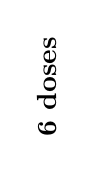
\begin{tikzpicture}
      \node[rotate=90] {\textbf{6 doses}};
    \end{tikzpicture}
  \end{subfigure}
  %
  \begin{subfigure}[c]{0.40\textwidth}
    \includegraphics[width=\textwidth]{figures/percentage-low-r2-curves-1-2-3-6doses-dil18-bowl-neg-controls-0.055.png}
  \end{subfigure}
  %
  \begin{subfigure}[c]{0.40\textwidth}
    \centering
    \includegraphics[width=\textwidth]{figures/percentage-low-r2-curves-1-2-3-6doses-dil18-bowl-neg-controls-0.085.png}
  \end{subfigure}

  \begin{subfigure}[c]{0.05\textwidth}
    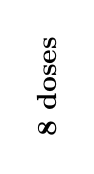
\begin{tikzpicture}
      \node[rotate=90] {\textbf{8 doses}};
    \end{tikzpicture}
  \end{subfigure}
  %
  \begin{subfigure}[c]{0.40\textwidth}
    \includegraphics[width=\textwidth]{figures/percentage-low-r2-curves-1-2-3-8doses-dil8-bowl-neg-controls-0.055.png}
  \end{subfigure}
  %
  \begin{subfigure}[c]{0.40\textwidth}
    \centering
    \includegraphics[width=\textwidth]{figures/percentage-low-r2-curves-1-2-3-8doses-dil8-bowl-neg-controls-0.085.png}
  \end{subfigure}

  \begin{subfigure}[c]{0.05\textwidth}
    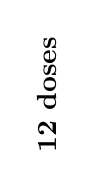
\begin{tikzpicture}
      \node[rotate=90] {\textbf{12 doses}};
    \end{tikzpicture}
  \end{subfigure}
  %
  \begin{subfigure}[c]{0.40\textwidth}
    \includegraphics[width=\textwidth]{figures/percentage-low-r2-curves-1-2-3-12doses-dil4-bowl-neg-controls-0.055.png}
  \end{subfigure}
  %
  \begin{subfigure}[c]{0.40\textwidth}
    \centering
    \includegraphics[width=\textwidth]{figures/percentage-low-r2-curves-1-2-3-12doses-dil4-bowl-neg-controls-0.085.png}
  \end{subfigure}

  \caption{Percentage of dose-response curves with low-quality ($R^2 < 80\%$) using various numbers of doses, replicates, and \emph{bowl-shaped} plate-effect strengths. The 4PL sigmoid curves were fitted using compound data and 4 negative controls such that their mean was equal to the mean of the 20 negative controls on the plate.}
\end{figure*}

\clearpage
\subsection{\emph{half-column} plate effects (column (half-plate))}


\subsubsection{$d_{\max}$ errors}

\begin{figure*}[!htbp]
  \centering
  \begin{subfigure}[c]{0.05\textwidth}
    ~
  \end{subfigure}
  %
  \begin{subfigure}[c]{0.40\textwidth}
    \centering
    ~~\textbf{Mild plate effects}
  \end{subfigure}
  %
  \begin{subfigure}[c]{0.40\textwidth}
    \centering
    ~~\textbf{Strong plate effects}
  \end{subfigure}

  \begin{subfigure}[c]{0.05\textwidth}
    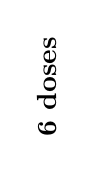
\begin{tikzpicture}
      \node[rotate=90] {\textbf{6 doses}};
    \end{tikzpicture}
  \end{subfigure}
  %
  \begin{subfigure}[c]{0.40\textwidth}
    \includegraphics[width=\textwidth]{figures/dose-response-d_diff-1-2-3-6doses-dil18-half-columns-neg-controls-0.2.png}
  \end{subfigure}
  %
  \begin{subfigure}[c]{0.40\textwidth}
    \centering
    \includegraphics[width=\textwidth]{figures/dose-response-d_diff-1-2-3-6doses-dil18-half-columns-neg-controls-0.4.png}
  \end{subfigure}

  \begin{subfigure}[c]{0.05\textwidth}
    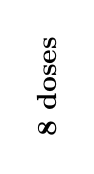
\begin{tikzpicture}
      \node[rotate=90] {\textbf{8 doses}};
    \end{tikzpicture}
  \end{subfigure}
  %
  \begin{subfigure}[c]{0.40\textwidth}
    \includegraphics[width=\textwidth]{figures/dose-response-d_diff-1-2-3-8doses-dil8-half-columns-neg-controls-0.2.png}
  \end{subfigure}
  %
  \begin{subfigure}[c]{0.40\textwidth}
    \centering
    \includegraphics[width=\textwidth]{figures/dose-response-d_diff-1-2-3-8doses-dil8-half-columns-neg-controls-0.4.png}
  \end{subfigure}

  \begin{subfigure}[c]{0.05\textwidth}
    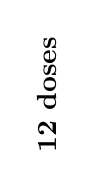
\begin{tikzpicture}
      \node[rotate=90] {\textbf{12 doses}};
    \end{tikzpicture}
  \end{subfigure}
  %
  \begin{subfigure}[c]{0.40\textwidth}
    \includegraphics[width=\textwidth]{figures/dose-response-d_diff-1-2-3-12doses-dil4-half-columns-neg-controls-0.2.png}
  \end{subfigure}
  %
  \begin{subfigure}[c]{0.40\textwidth}
    \centering
    \includegraphics[width=\textwidth]{figures/dose-response-d_diff-1-2-3-12doses-dil4-half-columns-neg-controls-0.4.png}
  \end{subfigure}

  \caption{Mean absolute difference between expected and obtained heights ($d_{\max}$) for dose-response curves using various numbers of doses, replicates, and \emph{half-column} plate-effect strengths. The 4PL sigmoid curves were fitted using compound data and 4 negative controls such that their mean was equal to the mean of the 20 negative controls on the plate. *** indicates $p\leq10^{-43}$.}
\end{figure*}

\begin{table}[H]
  \caption{%
    $d_{max}$ error overview for \emph{half-column} plate-effect strengths. Values are mean absolute differences in fitted $d_{max}$ across compounds. Best (lowest) value per row is \textbf{bolded}.
  }
  \label{tab:dr-overview-dmax-column}
  \centering
  \input{tables/dr-overview-dmax-column}
\end{table}


\clearpage
\subsubsection{Relative IC$_{50}$/EC$_{50}$ errors}

\begin{figure*}[!htbp]
  \centering
  \begin{subfigure}[c]{0.05\textwidth}
    ~
  \end{subfigure}
  %
  \begin{subfigure}[c]{0.40\textwidth}
    \centering
    ~~\textbf{Mild plate effects}
  \end{subfigure}
  %
  \begin{subfigure}[c]{0.40\textwidth}
    \centering
    ~~\textbf{Strong plate effects}
  \end{subfigure}

  \begin{subfigure}[c]{0.05\textwidth}
    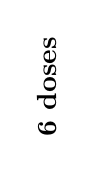
\begin{tikzpicture}
      \node[rotate=90] {\textbf{6 doses}};
    \end{tikzpicture}
  \end{subfigure}
  %
  \begin{subfigure}[c]{0.40\textwidth}
    \includegraphics[width=\textwidth]{figures/dose-response-relic50-1-2-3-6doses-dil18-half-columns-neg-controls-0.2.png}
  \end{subfigure}
  %
  \begin{subfigure}[c]{0.40\textwidth}
    \centering
    \includegraphics[width=\textwidth]{figures/dose-response-relic50-1-2-3-6doses-dil18-half-columns-neg-controls-0.4.png}
  \end{subfigure}

  \begin{subfigure}[c]{0.05\textwidth}
    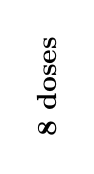
\begin{tikzpicture}
      \node[rotate=90] {\textbf{8 doses}};
    \end{tikzpicture}
  \end{subfigure}
  %
  \begin{subfigure}[c]{0.40\textwidth}
    \includegraphics[width=\textwidth]{figures/dose-response-relic50-1-2-3-8doses-dil8-half-columns-neg-controls-0.2.png}
  \end{subfigure}
  %
  \begin{subfigure}[c]{0.40\textwidth}
    \centering
    \includegraphics[width=\textwidth]{figures/dose-response-relic50-1-2-3-8doses-dil8-half-columns-neg-controls-0.4.png}
  \end{subfigure}

  \begin{subfigure}[c]{0.05\textwidth}
    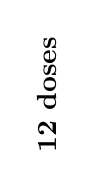
\begin{tikzpicture}
      \node[rotate=90] {\textbf{12 doses}};
    \end{tikzpicture}
  \end{subfigure}
  %
  \begin{subfigure}[c]{0.40\textwidth}
    \includegraphics[width=\textwidth]{figures/dose-response-relic50-1-2-3-12doses-dil4-half-columns-neg-controls-0.2.png}
  \end{subfigure}
  %
  \begin{subfigure}[c]{0.40\textwidth}
    \centering
    \includegraphics[width=\textwidth]{figures/dose-response-relic50-1-2-3-12doses-dil4-half-columns-neg-controls-0.4.png}
  \end{subfigure}

  \caption{Relative IC$_{50}$/EC$_{50}$ error for dose-response curves using various numbers of doses, replicates, and \emph{half-column} plate-effect strengths. *** indicates $p\leq10^{-43}$.}
\end{figure*}

\begin{table}[H]
  \caption{%
    Relative IC$_{50}$/EC$_{50}$ MSE overview for \emph{half-column} plate-effect strengths. Best (lowest) value per row is \textbf{bolded}.
  }
  \label{tab:dr-overview-rel-ic50-column}
  \centering
  \input{tables/dr-overview-rel-ic50-column}
\end{table}


\clearpage
\subsubsection{Absolute IC$_{50}$/EC$_{50}$ errors}

\begin{figure*}[!htbp]
  \centering
  \begin{subfigure}[c]{0.05\textwidth}
    ~
  \end{subfigure}
  %
  \begin{subfigure}[c]{0.40\textwidth}
    \centering
    ~~\textbf{Mild plate effects}
  \end{subfigure}
  %
  \begin{subfigure}[c]{0.40\textwidth}
    \centering
    ~~\textbf{Strong plate effects}
  \end{subfigure}

  \begin{subfigure}[c]{0.05\textwidth}
    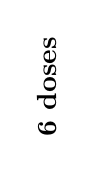
\begin{tikzpicture}
      \node[rotate=90] {\textbf{6 doses}};
    \end{tikzpicture}
  \end{subfigure}
  %
  \begin{subfigure}[c]{0.40\textwidth}
    \includegraphics[width=\textwidth]{figures/dose-response-absic50-1-2-3-6doses-dil18-half-columns-neg-controls-0.2.png}
  \end{subfigure}
  %
  \begin{subfigure}[c]{0.40\textwidth}
    \centering
    \includegraphics[width=\textwidth]{figures/dose-response-absic50-1-2-3-6doses-dil18-half-columns-neg-controls-0.4.png}
  \end{subfigure}

  \begin{subfigure}[c]{0.05\textwidth}
    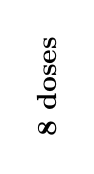
\begin{tikzpicture}
      \node[rotate=90] {\textbf{8 doses}};
    \end{tikzpicture}
  \end{subfigure}
  %
  \begin{subfigure}[c]{0.40\textwidth}
    \includegraphics[width=\textwidth]{figures/dose-response-absic50-1-2-3-8doses-dil8-half-columns-neg-controls-0.2.png}
  \end{subfigure}
  %
  \begin{subfigure}[c]{0.40\textwidth}
    \centering
    \includegraphics[width=\textwidth]{figures/dose-response-absic50-1-2-3-8doses-dil8-half-columns-neg-controls-0.4.png}
  \end{subfigure}

  \begin{subfigure}[c]{0.05\textwidth}
    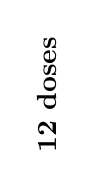
\begin{tikzpicture}
      \node[rotate=90] {\textbf{12 doses}};
    \end{tikzpicture}
  \end{subfigure}
  %
  \begin{subfigure}[c]{0.40\textwidth}
    \includegraphics[width=\textwidth]{figures/dose-response-absic50-1-2-3-12doses-dil4-half-columns-neg-controls-0.2.png}
  \end{subfigure}
  %
  \begin{subfigure}[c]{0.40\textwidth}
    \centering
    \includegraphics[width=\textwidth]{figures/dose-response-absic50-1-2-3-12doses-dil4-half-columns-neg-controls-0.4.png}
  \end{subfigure}

  \caption{Absolute IC$_{50}$/EC$_{50}$ error for dose-response curves using various numbers of doses, replicates, and \emph{half-column} plate-effect strengths. *** indicates $p\leq10^{-43}$.}
\end{figure*}

\begin{table}[H]
  \caption{%
    Absolute IC$_{50}$/EC$_{50}$ error overview for \emph{half-column} plate-effect strengths. Values are mean squared absolute IC$_{50}$/EC$_{50}$ estimation errors across compounds. Best (lowest) value per row is \textbf{bolded}.
  }
  \label{tab:dr-overview-abs-ic50-column}
  \centering
  \input{tables/dr-overview-abs-ic50-column}
\end{table}


\clearpage
\subsubsection{Residuals}

\begin{figure*}[!htbp]
  \centering
  \begin{subfigure}[c]{0.05\textwidth}
    ~
  \end{subfigure}
  %
  \begin{subfigure}[c]{0.40\textwidth}
    \centering
    ~~\textbf{Mild plate effects}
  \end{subfigure}
  %
  \begin{subfigure}[c]{0.40\textwidth}
    \centering
    ~~\textbf{Strong plate effects}
  \end{subfigure}

  \begin{subfigure}[c]{0.05\textwidth}
    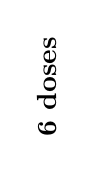
\begin{tikzpicture}
      \node[rotate=90] {\textbf{6 doses}};
    \end{tikzpicture}
  \end{subfigure}
  %
  \begin{subfigure}[c]{0.40\textwidth}
    \includegraphics[width=\textwidth]{figures/residuals-1-2-3-6doses-dil18-half-columns-neg-controls-0.2.png}
  \end{subfigure}
  %
  \begin{subfigure}[c]{0.40\textwidth}
    \centering
    \includegraphics[width=\textwidth]{figures/residuals-1-2-3-6doses-dil18-half-columns-neg-controls-0.4.png}
  \end{subfigure}

  \begin{subfigure}[c]{0.05\textwidth}
    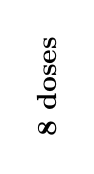
\begin{tikzpicture}
      \node[rotate=90] {\textbf{8 doses}};
    \end{tikzpicture}
  \end{subfigure}
  %
  \begin{subfigure}[c]{0.40\textwidth}
    \includegraphics[width=\textwidth]{figures/residuals-1-2-3-8doses-dil8-half-columns-neg-controls-0.2.png}
  \end{subfigure}
  %
  \begin{subfigure}[c]{0.40\textwidth}
    \centering
    \includegraphics[width=\textwidth]{figures/residuals-1-2-3-8doses-dil8-half-columns-neg-controls-0.4.png}
  \end{subfigure}

  \begin{subfigure}[c]{0.05\textwidth}
    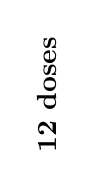
\begin{tikzpicture}
      \node[rotate=90] {\textbf{12 doses}};
    \end{tikzpicture}
  \end{subfigure}
  %
  \begin{subfigure}[c]{0.40\textwidth}
    \includegraphics[width=\textwidth]{figures/residuals-1-2-3-12doses-dil4-half-columns-neg-controls-0.2.png}
  \end{subfigure}
  %
  \begin{subfigure}[c]{0.40\textwidth}
    \centering
    \includegraphics[width=\textwidth]{figures/residuals-1-2-3-12doses-dil4-half-columns-neg-controls-0.4.png}
  \end{subfigure}

  \caption{Residuals (MSE between expected and obtained responses) for dose-response simulations using various numbers of doses, replicates, and \emph{half-column} plate-effect strengths. *** indicates $p\leq10^{-43}$.}
\end{figure*}

\begin{table}[H]
  \caption{%
    Residual MSE overview for \emph{half-column} plate-effect strengths. Best (lowest) value per row is \textbf{bolded}.
  }
  \label{tab:dr-overview-residuals-column}
  \centering
  \input{tables/dr-overview-residuals-column}
\end{table}


\clearpage
\subsection{\emph{row-gradient} plate effects (row gradient (top-to-bottom))}


\subsubsection{$d_{\max}$ errors}

\begin{figure*}[!htbp]
  \centering
  \begin{subfigure}[c]{0.05\textwidth}
    ~
  \end{subfigure}
  %
  \begin{subfigure}[c]{0.40\textwidth}
    \centering
    ~~\textbf{Mild plate effects}
  \end{subfigure}
  %
  \begin{subfigure}[c]{0.40\textwidth}
    \centering
    ~~\textbf{Strong plate effects}
  \end{subfigure}

  \begin{subfigure}[c]{0.05\textwidth}
    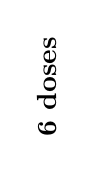
\begin{tikzpicture}
      \node[rotate=90] {\textbf{6 doses}};
    \end{tikzpicture}
  \end{subfigure}
  %
  \begin{subfigure}[c]{0.40\textwidth}
    \includegraphics[width=\textwidth]{figures/dose-response-d_diff-1-2-3-6doses-dil18-row-gradient-0.006.png}
  \end{subfigure}
  %
  \begin{subfigure}[c]{0.40\textwidth}
    \centering
    \includegraphics[width=\textwidth]{figures/dose-response-d_diff-1-2-3-6doses-dil18-row-gradient-0.012.png}
  \end{subfigure}

  \begin{subfigure}[c]{0.05\textwidth}
    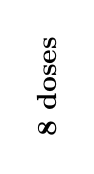
\begin{tikzpicture}
      \node[rotate=90] {\textbf{8 doses}};
    \end{tikzpicture}
  \end{subfigure}
  %
  \begin{subfigure}[c]{0.40\textwidth}
    \includegraphics[width=\textwidth]{figures/dose-response-d_diff-1-2-3-8doses-dil8-row-gradient-0.006.png}
  \end{subfigure}
  %
  \begin{subfigure}[c]{0.40\textwidth}
    \centering
    \includegraphics[width=\textwidth]{figures/dose-response-d_diff-1-2-3-8doses-dil8-row-gradient-0.012.png}
  \end{subfigure}

  \begin{subfigure}[c]{0.05\textwidth}
    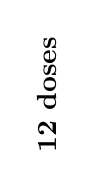
\begin{tikzpicture}
      \node[rotate=90] {\textbf{12 doses}};
    \end{tikzpicture}
  \end{subfigure}
  %
  \begin{subfigure}[c]{0.40\textwidth}
    \includegraphics[width=\textwidth]{figures/dose-response-d_diff-1-2-3-12doses-dil4-row-gradient-0.006.png}
  \end{subfigure}
  %
  \begin{subfigure}[c]{0.40\textwidth}
    \centering
    \includegraphics[width=\textwidth]{figures/dose-response-d_diff-1-2-3-12doses-dil4-row-gradient-0.012.png}
  \end{subfigure}

  \caption{Mean absolute difference between expected and obtained heights ($d_{\max}$) for dose-response curves using various numbers of doses, replicates, and \emph{row-gradient} plate-effect strengths. The 4PL sigmoid curves were fitted using compound data and 4 negative controls such that their mean was equal to the mean of the 20 negative controls on the plate. *** indicates $p\leq10^{-43}$.}
\end{figure*}

\begin{table}[H]
  \caption{%
    $d_{max}$ error overview for \emph{row-gradient} plate-effect strengths. Values are mean absolute differences in fitted $d_{max}$ across compounds. Best (lowest) value per row is \textbf{bolded}.
  }
  \label{tab:dr-overview-dmax-row-gradient}
  \centering
  \input{tables/dr-overview-dmax-row-gradient}
\end{table}


\clearpage
\subsubsection{Relative IC$_{50}$/EC$_{50}$ errors}

\begin{figure*}[!htbp]
  \centering
  \begin{subfigure}[c]{0.05\textwidth}
    ~
  \end{subfigure}
  %
  \begin{subfigure}[c]{0.40\textwidth}
    \centering
    ~~\textbf{Mild plate effects}
  \end{subfigure}
  %
  \begin{subfigure}[c]{0.40\textwidth}
    \centering
    ~~\textbf{Strong plate effects}
  \end{subfigure}

  \begin{subfigure}[c]{0.05\textwidth}
    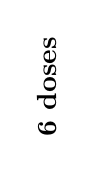
\begin{tikzpicture}
      \node[rotate=90] {\textbf{6 doses}};
    \end{tikzpicture}
  \end{subfigure}
  %
  \begin{subfigure}[c]{0.40\textwidth}
    \includegraphics[width=\textwidth]{figures/dose-response-relic50-1-2-3-6doses-dil18-row-gradient-0.006.png}
  \end{subfigure}
  %
  \begin{subfigure}[c]{0.40\textwidth}
    \centering
    \includegraphics[width=\textwidth]{figures/dose-response-relic50-1-2-3-6doses-dil18-row-gradient-0.012.png}
  \end{subfigure}

  \begin{subfigure}[c]{0.05\textwidth}
    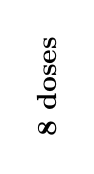
\begin{tikzpicture}
      \node[rotate=90] {\textbf{8 doses}};
    \end{tikzpicture}
  \end{subfigure}
  %
  \begin{subfigure}[c]{0.40\textwidth}
    \includegraphics[width=\textwidth]{figures/dose-response-relic50-1-2-3-8doses-dil8-row-gradient-0.006.png}
  \end{subfigure}
  %
  \begin{subfigure}[c]{0.40\textwidth}
    \centering
    \includegraphics[width=\textwidth]{figures/dose-response-relic50-1-2-3-8doses-dil8-row-gradient-0.012.png}
  \end{subfigure}

  \begin{subfigure}[c]{0.05\textwidth}
    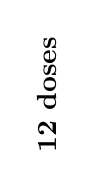
\begin{tikzpicture}
      \node[rotate=90] {\textbf{12 doses}};
    \end{tikzpicture}
  \end{subfigure}
  %
  \begin{subfigure}[c]{0.40\textwidth}
    \includegraphics[width=\textwidth]{figures/dose-response-relic50-1-2-3-12doses-dil4-row-gradient-0.006.png}
  \end{subfigure}
  %
  \begin{subfigure}[c]{0.40\textwidth}
    \centering
    \includegraphics[width=\textwidth]{figures/dose-response-relic50-1-2-3-12doses-dil4-row-gradient-0.012.png}
  \end{subfigure}

  \caption{Relative IC$_{50}$/EC$_{50}$ error for dose-response curves using various numbers of doses, replicates, and \emph{row-gradient} plate-effect strengths. *** indicates $p\leq10^{-43}$.}
\end{figure*}

\begin{table}[H]
  \caption{%
    Relative IC$_{50}$/EC$_{50}$ MSE overview for \emph{row-gradient} plate-effect strengths. Best (lowest) value per row is \textbf{bolded}.
  }
  \label{tab:dr-overview-rel-ic50-row-gradient}
  \centering
  \input{tables/dr-overview-rel-ic50-row-gradient}
\end{table}


\clearpage
\subsubsection{Absolute IC$_{50}$/EC$_{50}$ errors}

\begin{figure*}[!htbp]
  \centering
  \begin{subfigure}[c]{0.05\textwidth}
    ~
  \end{subfigure}
  %
  \begin{subfigure}[c]{0.40\textwidth}
    \centering
    ~~\textbf{Mild plate effects}
  \end{subfigure}
  %
  \begin{subfigure}[c]{0.40\textwidth}
    \centering
    ~~\textbf{Strong plate effects}
  \end{subfigure}

  \begin{subfigure}[c]{0.05\textwidth}
    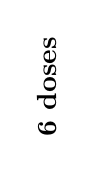
\begin{tikzpicture}
      \node[rotate=90] {\textbf{6 doses}};
    \end{tikzpicture}
  \end{subfigure}
  %
  \begin{subfigure}[c]{0.40\textwidth}
    \includegraphics[width=\textwidth]{figures/dose-response-absic50-1-2-3-6doses-dil18-row-gradient-0.006.png}
  \end{subfigure}
  %
  \begin{subfigure}[c]{0.40\textwidth}
    \centering
    \includegraphics[width=\textwidth]{figures/dose-response-absic50-1-2-3-6doses-dil18-row-gradient-0.012.png}
  \end{subfigure}

  \begin{subfigure}[c]{0.05\textwidth}
    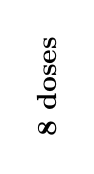
\begin{tikzpicture}
      \node[rotate=90] {\textbf{8 doses}};
    \end{tikzpicture}
  \end{subfigure}
  %
  \begin{subfigure}[c]{0.40\textwidth}
    \includegraphics[width=\textwidth]{figures/dose-response-absic50-1-2-3-8doses-dil8-row-gradient-0.006.png}
  \end{subfigure}
  %
  \begin{subfigure}[c]{0.40\textwidth}
    \centering
    \includegraphics[width=\textwidth]{figures/dose-response-absic50-1-2-3-8doses-dil8-row-gradient-0.012.png}
  \end{subfigure}

  \begin{subfigure}[c]{0.05\textwidth}
    \begin{tikzpicture}
      \node[rotate=90] {\textbf{12 doses}};
    \end{tikzpicture}
  \end{subfigure}
  %
  \begin{subfigure}[c]{0.40\textwidth}
    \includegraphics[width=\textwidth]{figures/dose-response-absic50-1-2-3-12doses-dil4-row-gradient-0.006.png}
  \end{subfigure}
  %
  \begin{subfigure}[c]{0.40\textwidth}
    \centering
    \includegraphics[width=\textwidth]{figures/dose-response-absic50-1-2-3-12doses-dil4-row-gradient-0.012.png}
  \end{subfigure}

  \caption{Absolute IC$_{50}$/EC$_{50}$ error for dose-response curves using various numbers of doses, replicates, and \emph{row-gradient} plate-effect strengths. *** indicates $p\leq10^{-43}$.}
\end{figure*}

\begin{table}[H]
  \caption{%
    Absolute IC$_{50}$/EC$_{50}$ error overview for \emph{row-gradient} plate-effect strengths. Values are mean squared absolute IC$_{50}$/EC$_{50}$ estimation errors across compounds. Best (lowest) value per row is \textbf{bolded}.
  }
  \label{tab:dr-overview-abs-ic50-row-gradient}
  \centering
  \input{tables/dr-overview-abs-ic50-row-gradient}
\end{table}


\clearpage
\subsubsection{Residuals}

\begin{figure*}[!htbp]
  \centering
  \begin{subfigure}[c]{0.05\textwidth}
    ~
  \end{subfigure}
  %
  \begin{subfigure}[c]{0.40\textwidth}
    \centering
    ~~\textbf{Mild plate effects}
  \end{subfigure}
  %
  \begin{subfigure}[c]{0.40\textwidth}
    \centering
    ~~\textbf{Strong plate effects}
  \end{subfigure}

  \begin{subfigure}[c]{0.05\textwidth}
    \begin{tikzpicture}
      \node[rotate=90] {\textbf{6 doses}};
    \end{tikzpicture}
  \end{subfigure}
  %
  \begin{subfigure}[c]{0.40\textwidth}
    \includegraphics[width=\textwidth]{figures/residuals-1-2-3-6doses-dil18-row-gradient-0.006.png}
  \end{subfigure}
  %
  \begin{subfigure}[c]{0.40\textwidth}
    \centering
    \includegraphics[width=\textwidth]{figures/residuals-1-2-3-6doses-dil18-row-gradient-0.012.png}
  \end{subfigure}

  \begin{subfigure}[c]{0.05\textwidth}
    \begin{tikzpicture}
      \node[rotate=90] {\textbf{8 doses}};
    \end{tikzpicture}
  \end{subfigure}
  %
  \begin{subfigure}[c]{0.40\textwidth}
    \includegraphics[width=\textwidth]{figures/residuals-1-2-3-8doses-dil8-row-gradient-0.006.png}
  \end{subfigure}
  %
  \begin{subfigure}[c]{0.40\textwidth}
    \centering
    \includegraphics[width=\textwidth]{figures/residuals-1-2-3-8doses-dil8-row-gradient-0.012.png}
  \end{subfigure}

  \begin{subfigure}[c]{0.05\textwidth}
    \begin{tikzpicture}
      \node[rotate=90] {\textbf{12 doses}};
    \end{tikzpicture}
  \end{subfigure}
  %
  \begin{subfigure}[c]{0.40\textwidth}
    \includegraphics[width=\textwidth]{figures/residuals-1-2-3-12doses-dil4-row-gradient-0.006.png}
  \end{subfigure}
  %
  \begin{subfigure}[c]{0.40\textwidth}
    \centering
    \includegraphics[width=\textwidth]{figures/residuals-1-2-3-12doses-dil4-row-gradient-0.012.png}
  \end{subfigure}

  \caption{Residuals (MSE between expected and obtained responses) for dose-response simulations using various numbers of doses, replicates, and \emph{row-gradient} plate-effect strengths. *** indicates $p\leq10^{-43}$.}
\end{figure*}

\begin{table}[H]
  \caption{%
    Residual MSE overview for \emph{row-gradient} plate-effect strengths. Best (lowest) value per row is \textbf{bolded}.
  }
  \label{tab:dr-overview-residuals-row-gradient}
  \centering
  \input{tables/dr-overview-residuals-row-gradient}
\end{table}


\clearpage
\subsubsection{Fraction of poor fits (low $R^2$)}

\begin{figure*}[!htbp]
  \centering
  \begin{subfigure}[c]{0.05\textwidth}
    ~
  \end{subfigure}
  %
  \begin{subfigure}[c]{0.40\textwidth}
    \centering
    ~~\textbf{Mild plate effects}
  \end{subfigure}
  %
  \begin{subfigure}[c]{0.40\textwidth}
    \centering
    ~~\textbf{Strong plate effects}
  \end{subfigure}

  \begin{subfigure}[c]{0.05\textwidth}
    \begin{tikzpicture}
      \node[rotate=90] {\textbf{6 doses}};
    \end{tikzpicture}
  \end{subfigure}
  %
  \begin{subfigure}[c]{0.40\textwidth}
    \includegraphics[width=\textwidth]{figures/percentage-low-r2-curves-1-2-3-6doses-dil18-row-gradient-0.006.png}
  \end{subfigure}
  %
  \begin{subfigure}[c]{0.40\textwidth}
    \centering
    \includegraphics[width=\textwidth]{figures/percentage-low-r2-curves-1-2-3-6doses-dil18-row-gradient-0.012.png}
  \end{subfigure}

  \begin{subfigure}[c]{0.05\textwidth}
    \begin{tikzpicture}
      \node[rotate=90] {\textbf{8 doses}};
    \end{tikzpicture}
  \end{subfigure}
  %
  \begin{subfigure}[c]{0.40\textwidth}
    \includegraphics[width=\textwidth]{figures/percentage-low-r2-curves-1-2-3-8doses-dil8-row-gradient-0.006.png}
  \end{subfigure}
  %
  \begin{subfigure}[c]{0.40\textwidth}
    \centering
    \includegraphics[width=\textwidth]{figures/percentage-low-r2-curves-1-2-3-8doses-dil8-row-gradient-0.012.png}
  \end{subfigure}

  \begin{subfigure}[c]{0.05\textwidth}
    \begin{tikzpicture}
      \node[rotate=90] {\textbf{12 doses}};
    \end{tikzpicture}
  \end{subfigure}
  %
  \begin{subfigure}[c]{0.40\textwidth}
    \includegraphics[width=\textwidth]{figures/percentage-low-r2-curves-1-2-3-12doses-dil4-row-gradient-0.006.png}
  \end{subfigure}
  %
  \begin{subfigure}[c]{0.40\textwidth}
    \centering
    \includegraphics[width=\textwidth]{figures/percentage-low-r2-curves-1-2-3-12doses-dil4-row-gradient-0.012.png}
  \end{subfigure}

  \caption{Percentage of dose-response curves with low-quality ($R^2 < 80\%$) using various numbers of doses, replicates, and \emph{row-gradient} plate-effect strengths. The 4PL sigmoid curves were fitted using compound data and 4 negative controls such that their mean was equal to the mean of the 20 negative controls on the plate.}
\end{figure*}

\clearpage
\subsection{\emph{striped-row} plate effects (row stripe (even rows elevated))}


\subsubsection{$d_{\max}$ errors}

\begin{figure*}[!htbp]
  \centering
  \begin{subfigure}[c]{0.05\textwidth}
    ~
  \end{subfigure}
  %
  \begin{subfigure}[c]{0.40\textwidth}
    \centering
    ~~\textbf{Mild plate effects}
  \end{subfigure}
  %
  \begin{subfigure}[c]{0.40\textwidth}
    \centering
    ~~\textbf{Strong plate effects}
  \end{subfigure}

  \begin{subfigure}[c]{0.05\textwidth}
    \begin{tikzpicture}
      \node[rotate=90] {\textbf{6 doses}};
    \end{tikzpicture}
  \end{subfigure}
  %
  \begin{subfigure}[c]{0.40\textwidth}
    \includegraphics[width=\textwidth]{figures/dose-response-d_diff-1-2-3-6doses-dil18-striped-row-even-0.05.png}
  \end{subfigure}
  %
  \begin{subfigure}[c]{0.40\textwidth}
    \centering
    \includegraphics[width=\textwidth]{figures/dose-response-d_diff-1-2-3-6doses-dil18-striped-row-even-0.1.png}
  \end{subfigure}

  \begin{subfigure}[c]{0.05\textwidth}
    \begin{tikzpicture}
      \node[rotate=90] {\textbf{8 doses}};
    \end{tikzpicture}
  \end{subfigure}
  %
  \begin{subfigure}[c]{0.40\textwidth}
    \includegraphics[width=\textwidth]{figures/dose-response-d_diff-1-2-3-8doses-dil8-striped-row-even-0.05.png}
  \end{subfigure}
  %
  \begin{subfigure}[c]{0.40\textwidth}
    \centering
    \includegraphics[width=\textwidth]{figures/dose-response-d_diff-1-2-3-8doses-dil8-striped-row-even-0.1.png}
  \end{subfigure}

  \begin{subfigure}[c]{0.05\textwidth}
    \begin{tikzpicture}
      \node[rotate=90] {\textbf{12 doses}};
    \end{tikzpicture}
  \end{subfigure}
  %
  \begin{subfigure}[c]{0.40\textwidth}
    \includegraphics[width=\textwidth]{figures/dose-response-d_diff-1-2-3-12doses-dil4-striped-row-even-0.05.png}
  \end{subfigure}
  %
  \begin{subfigure}[c]{0.40\textwidth}
    \centering
    \includegraphics[width=\textwidth]{figures/dose-response-d_diff-1-2-3-12doses-dil4-striped-row-even-0.1.png}
  \end{subfigure}

  \caption{Mean absolute difference between expected and obtained heights ($d_{\max}$) for dose-response curves using various numbers of doses, replicates, and \emph{striped-row} plate-effect strengths. The 4PL sigmoid curves were fitted using compound data and 4 negative controls such that their mean was equal to the mean of the 20 negative controls on the plate. *** indicates $p\leq10^{-43}$.}
\end{figure*}

\begin{table}[H]
  \caption{%
    $d_{max}$ error overview for \emph{striped-row} plate-effect strengths. Values are mean absolute differences in fitted $d_{max}$ across compounds. Best (lowest) value per row is \textbf{bolded}.
  }
  \label{tab:dr-overview-dmax-striped-row-even}
  \centering
  \input{tables/dr-overview-dmax-striped-row-even}
\end{table}


\clearpage
\subsubsection{Relative IC$_{50}$/EC$_{50}$ errors}

\begin{figure*}[!htbp]
  \centering
  \begin{subfigure}[c]{0.05\textwidth}
    ~
  \end{subfigure}
  %
  \begin{subfigure}[c]{0.40\textwidth}
    \centering
    ~~\textbf{Mild plate effects}
  \end{subfigure}
  %
  \begin{subfigure}[c]{0.40\textwidth}
    \centering
    ~~\textbf{Strong plate effects}
  \end{subfigure}

  \begin{subfigure}[c]{0.05\textwidth}
    \begin{tikzpicture}
      \node[rotate=90] {\textbf{6 doses}};
    \end{tikzpicture}
  \end{subfigure}
  %
  \begin{subfigure}[c]{0.40\textwidth}
    \includegraphics[width=\textwidth]{figures/dose-response-relic50-1-2-3-6doses-dil18-striped-row-even-0.05.png}
  \end{subfigure}
  %
  \begin{subfigure}[c]{0.40\textwidth}
    \centering
    \includegraphics[width=\textwidth]{figures/dose-response-relic50-1-2-3-6doses-dil18-striped-row-even-0.1.png}
  \end{subfigure}

  \begin{subfigure}[c]{0.05\textwidth}
    \begin{tikzpicture}
      \node[rotate=90] {\textbf{8 doses}};
    \end{tikzpicture}
  \end{subfigure}
  %
  \begin{subfigure}[c]{0.40\textwidth}
    \includegraphics[width=\textwidth]{figures/dose-response-relic50-1-2-3-8doses-dil8-striped-row-even-0.05.png}
  \end{subfigure}
  %
  \begin{subfigure}[c]{0.40\textwidth}
    \centering
    \includegraphics[width=\textwidth]{figures/dose-response-relic50-1-2-3-8doses-dil8-striped-row-even-0.1.png}
  \end{subfigure}

  \begin{subfigure}[c]{0.05\textwidth}
    \begin{tikzpicture}
      \node[rotate=90] {\textbf{12 doses}};
    \end{tikzpicture}
  \end{subfigure}
  %
  \begin{subfigure}[c]{0.40\textwidth}
    \includegraphics[width=\textwidth]{figures/dose-response-relic50-1-2-3-12doses-dil4-striped-row-even-0.05.png}
  \end{subfigure}
  %
  \begin{subfigure}[c]{0.40\textwidth}
    \centering
    \includegraphics[width=\textwidth]{figures/dose-response-relic50-1-2-3-12doses-dil4-striped-row-even-0.1.png}
  \end{subfigure}

  \caption{Relative IC$_{50}$/EC$_{50}$ error for dose-response curves using various numbers of doses, replicates, and \emph{striped-row} plate-effect strengths. *** indicates $p\leq10^{-43}$.}
\end{figure*}

\begin{table}[H]
  \caption{%
    Relative IC$_{50}$/EC$_{50}$ MSE overview for \emph{striped-row} plate-effect strengths. Best (lowest) value per row is \textbf{bolded}.
  }
  \label{tab:dr-overview-rel-ic50-striped-row-even}
  \centering
  \input{tables/dr-overview-rel-ic50-striped-row-even}
\end{table}


\clearpage
\subsubsection{Absolute IC$_{50}$/EC$_{50}$ errors}

\begin{figure*}[!htbp]
  \centering
  \begin{subfigure}[c]{0.05\textwidth}
    ~
  \end{subfigure}
  %
  \begin{subfigure}[c]{0.40\textwidth}
    \centering
    ~~\textbf{Mild plate effects}
  \end{subfigure}
  %
  \begin{subfigure}[c]{0.40\textwidth}
    \centering
    ~~\textbf{Strong plate effects}
  \end{subfigure}

  \begin{subfigure}[c]{0.05\textwidth}
    \begin{tikzpicture}
      \node[rotate=90] {\textbf{6 doses}};
    \end{tikzpicture}
  \end{subfigure}
  %
  \begin{subfigure}[c]{0.40\textwidth}
    \includegraphics[width=\textwidth]{figures/dose-response-absic50-1-2-3-6doses-dil18-striped-row-even-0.05.png}
  \end{subfigure}
  %
  \begin{subfigure}[c]{0.40\textwidth}
    \centering
    \includegraphics[width=\textwidth]{figures/dose-response-absic50-1-2-3-6doses-dil18-striped-row-even-0.1.png}
  \end{subfigure}

  \begin{subfigure}[c]{0.05\textwidth}
    \begin{tikzpicture}
      \node[rotate=90] {\textbf{8 doses}};
    \end{tikzpicture}
  \end{subfigure}
  %
  \begin{subfigure}[c]{0.40\textwidth}
    \includegraphics[width=\textwidth]{figures/dose-response-absic50-1-2-3-8doses-dil8-striped-row-even-0.05.png}
  \end{subfigure}
  %
  \begin{subfigure}[c]{0.40\textwidth}
    \centering
    \includegraphics[width=\textwidth]{figures/dose-response-absic50-1-2-3-8doses-dil8-striped-row-even-0.1.png}
  \end{subfigure}

  \begin{subfigure}[c]{0.05\textwidth}
    \begin{tikzpicture}
      \node[rotate=90] {\textbf{12 doses}};
    \end{tikzpicture}
  \end{subfigure}
  %
  \begin{subfigure}[c]{0.40\textwidth}
    \includegraphics[width=\textwidth]{figures/dose-response-absic50-1-2-3-12doses-dil4-striped-row-even-0.05.png}
  \end{subfigure}
  %
  \begin{subfigure}[c]{0.40\textwidth}
    \centering
    \includegraphics[width=\textwidth]{figures/dose-response-absic50-1-2-3-12doses-dil4-striped-row-even-0.1.png}
  \end{subfigure}

  \caption{Absolute IC$_{50}$/EC$_{50}$ error for dose-response curves using various numbers of doses, replicates, and \emph{striped-row} plate-effect strengths. *** indicates $p\leq10^{-43}$.}
\end{figure*}

\begin{table}[H]
  \caption{%
    Absolute IC$_{50}$/EC$_{50}$ error overview for \emph{striped-row} plate-effect strengths. Values are mean squared absolute IC$_{50}$/EC$_{50}$ estimation errors across compounds. Best (lowest) value per row is \textbf{bolded}.
  }
  \label{tab:dr-overview-abs-ic50-striped-row-even}
  \centering
  \input{tables/dr-overview-abs-ic50-striped-row-even}
\end{table}


\clearpage
\subsubsection{Residuals}

\begin{figure*}[!htbp]
  \centering
  \begin{subfigure}[c]{0.05\textwidth}
    ~
  \end{subfigure}
  %
  \begin{subfigure}[c]{0.40\textwidth}
    \centering
    ~~\textbf{Mild plate effects}
  \end{subfigure}
  %
  \begin{subfigure}[c]{0.40\textwidth}
    \centering
    ~~\textbf{Strong plate effects}
  \end{subfigure}

  \begin{subfigure}[c]{0.05\textwidth}
    \begin{tikzpicture}
      \node[rotate=90] {\textbf{6 doses}};
    \end{tikzpicture}
  \end{subfigure}
  %
  \begin{subfigure}[c]{0.40\textwidth}
    \includegraphics[width=\textwidth]{figures/residuals-1-2-3-6doses-dil18-striped-row-even-0.05.png}
  \end{subfigure}
  %
  \begin{subfigure}[c]{0.40\textwidth}
    \centering
    \includegraphics[width=\textwidth]{figures/residuals-1-2-3-6doses-dil18-striped-row-even-0.1.png}
  \end{subfigure}

  \begin{subfigure}[c]{0.05\textwidth}
    \begin{tikzpicture}
      \node[rotate=90] {\textbf{8 doses}};
    \end{tikzpicture}
  \end{subfigure}
  %
  \begin{subfigure}[c]{0.40\textwidth}
    \includegraphics[width=\textwidth]{figures/residuals-1-2-3-8doses-dil8-striped-row-even-0.05.png}
  \end{subfigure}
  %
  \begin{subfigure}[c]{0.40\textwidth}
    \centering
    \includegraphics[width=\textwidth]{figures/residuals-1-2-3-8doses-dil8-striped-row-even-0.1.png}
  \end{subfigure}

  \begin{subfigure}[c]{0.05\textwidth}
    \begin{tikzpicture}
      \node[rotate=90] {\textbf{12 doses}};
    \end{tikzpicture}
  \end{subfigure}
  %
  \begin{subfigure}[c]{0.40\textwidth}
    \includegraphics[width=\textwidth]{figures/residuals-1-2-3-12doses-dil4-striped-row-even-0.05.png}
  \end{subfigure}
  %
  \begin{subfigure}[c]{0.40\textwidth}
    \centering
    \includegraphics[width=\textwidth]{figures/residuals-1-2-3-12doses-dil4-striped-row-even-0.1.png}
  \end{subfigure}

  \caption{Residuals (MSE between expected and obtained responses) for dose-response simulations using various numbers of doses, replicates, and \emph{striped-row} plate-effect strengths. *** indicates $p\leq10^{-43}$.}
\end{figure*}

\begin{table}[H]
  \caption{%
    Residual MSE overview for \emph{striped-row} plate-effect strengths. Best (lowest) value per row is \textbf{bolded}.
  }
  \label{tab:dr-overview-residuals-striped-row-even}
  \centering
  \input{tables/dr-overview-residuals-striped-row-even}
\end{table}


\clearpage
\subsubsection{Fraction of poor fits (low $R^2$)}

\begin{figure*}[!htbp]
  \centering
  \begin{subfigure}[c]{0.05\textwidth}
    ~
  \end{subfigure}
  %
  \begin{subfigure}[c]{0.40\textwidth}
    \centering
    ~~\textbf{Mild plate effects}
  \end{subfigure}
  %
  \begin{subfigure}[c]{0.40\textwidth}
    \centering
    ~~\textbf{Strong plate effects}
  \end{subfigure}

  \begin{subfigure}[c]{0.05\textwidth}
    \begin{tikzpicture}
      \node[rotate=90] {\textbf{6 doses}};
    \end{tikzpicture}
  \end{subfigure}
  %
  \begin{subfigure}[c]{0.40\textwidth}
    \includegraphics[width=\textwidth]{figures/percentage-low-r2-curves-1-2-3-6doses-dil18-striped-row-even-0.05.png}
  \end{subfigure}
  %
  \begin{subfigure}[c]{0.40\textwidth}
    \centering
    \includegraphics[width=\textwidth]{figures/percentage-low-r2-curves-1-2-3-6doses-dil18-striped-row-even-0.1.png}
  \end{subfigure}

  \begin{subfigure}[c]{0.05\textwidth}
    \begin{tikzpicture}
      \node[rotate=90] {\textbf{8 doses}};
    \end{tikzpicture}
  \end{subfigure}
  %
  \begin{subfigure}[c]{0.40\textwidth}
    \includegraphics[width=\textwidth]{figures/percentage-low-r2-curves-1-2-3-8doses-dil8-striped-row-even-0.05.png}
  \end{subfigure}
  %
  \begin{subfigure}[c]{0.40\textwidth}
    \centering
    \includegraphics[width=\textwidth]{figures/percentage-low-r2-curves-1-2-3-8doses-dil8-striped-row-even-0.1.png}
  \end{subfigure}

  \begin{subfigure}[c]{0.05\textwidth}
    \begin{tikzpicture}
      \node[rotate=90] {\textbf{12 doses}};
    \end{tikzpicture}
  \end{subfigure}
  %
  \begin{subfigure}[c]{0.40\textwidth}
    \includegraphics[width=\textwidth]{figures/percentage-low-r2-curves-1-2-3-12doses-dil4-striped-row-even-0.05.png}
  \end{subfigure}
  %
  \begin{subfigure}[c]{0.40\textwidth}
    \centering
    \includegraphics[width=\textwidth]{figures/percentage-low-r2-curves-1-2-3-12doses-dil4-striped-row-even-0.1.png}
  \end{subfigure}

  \caption{Percentage of dose-response curves with low-quality ($R^2 < 80\%$) using various numbers of doses, replicates, and \emph{striped-row} plate-effect strengths. The 4PL sigmoid curves were fitted using compound data and 4 negative controls such that their mean was equal to the mean of the 20 negative controls on the plate.}
\end{figure*}
